\documentclass[a4paper,10pt]{article}
\usepackage[utf8]{inputenc}
\usepackage[spanish]{babel}
\usepackage[hmargin=2.5cm, vmargin=2.5cm]{geometry}
\usepackage{amsmath}
\usepackage{graphicx}
\usepackage{natbib}
\usepackage{url}
\usepackage[pdftex,colorlinks=true]{hyperref}
\hypersetup{
    allcolors=black,
}
\usepackage{mathptmx} %Times font


\title{
    \textbf{
    TESSEROIDES CON DENSIDADES VARIABLES:
    CÁLCULO DE CAMPOS GRAVITATORIOS EN COORDENADAS ESFÉRICAS CON
    DENSIDADES VARIABLES EN PROFUNDIDAD
    }
}
\author{
    Santiago R. Soler$^{1,2}$ \vspace{0.5em} \\ 
    \textit{$^1$ Instituto Geofísico Sismológico Volponi, Universidad Nacional de San Juan} \\
    \textit{$^2$ Consejo Nacional de Investigaciones Científicas y Técnicas (CONICET)} \vspace{0.4em} \\
    email: santiago.r.soler@gmail.com
}
\date{}


\begin{document}

\maketitle

\vspace{-2.5em}
\begin{center}
\textbf{Palabras Clave:} poner algo
\end{center}
\vspace{0.5em}

\begin{abstract}
El cálculo directo de campos gravitatorios para grandes extensiones requiere tomar en cuenta la curvatura de la Tierra, lo cual suele resolverse a través del uso de prismas esféricos llamados Tesseroides. Además, estructuras como cuencas sedimentarias presentan variaciones de densidad con la profundidad.

\end{abstract}


\section{Introducción}

Las variaciones de la densidad en la corteza con la profundidad han sido estudiadas por casi un siglo: se propusieron diferentes tipos de variaciones con la profundidad \citep{Athy1930, Maxant1980, Rao1986, Rao1993, Rao1994} e incluso se han tenido en cuenta en modelos directos y de inversión gravimétrica, principalmente aplicados en cuencas y fosas \citep{Cordell1973, Rao1986, Cowie1990, Rao1993, Rao1994, Zhang2001, Welford2010}.

Estos modelos directos fueron desarrollados para cuerpos bidimensionales o tridimensionales en coordenadas cartesianas, los cuales se ajustan adecuadamente para aplicaciones de escalas locales.
Sin embargo, la disponibilidad de datos gravimétricos satelitales permite llevar a cabo estudios e interpretaciones a escalas regionales, en las cuales es necesario tomar en cuenta la curvatura de la Tierra a la hora de realizar modelados directos. 

\begin{figure}
\centering
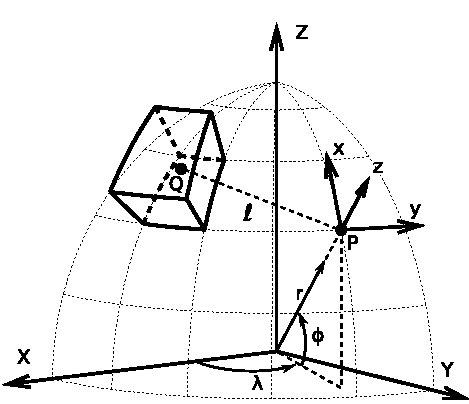
\includegraphics[width=0.4\linewidth]{../manuscript/figures/tesseroid-uieda.pdf}
\caption{
Prisma esférico, también conocido como Tesseroid, en un sistema geocéntrico de coordenadas esféricas, junto a un punto de cómputo $P$ y su respectivo sistema de coordenadas Cartesiano local orientado hacia el Norte. Imágen producida por \citet{Uieda2015}.
}
\label{fig:tesseroid-uieda}
\end{figure}

Un método muy común para hacerlo es discretizar la Tierra en prismas esféricos conocidos como Tesseroids (ver Figura \ref{fig:tesseroid-uieda}).
El cómputo de campos gravitatorios generados por un tesseroid arbitrario en un punto externo al mismo involucra la resolución de integrales volumétricas.
En caso de que el tesseroid posea una densidad variable, las ecuaciones obtenidas por \citet{Grombein2013} \citep[ver también][]{Uieda2016} para el cómputo de los campos gravitatorios se ven ligeramente modificadas. Por ejemplo, el potencial generado por un tesseroid arbitrario con densidad $\rho(r')$ sobre un punto de cómputo $P(r, \phi, \lambda)$ se puede obtener como:

\begin{equation}
    V(r,\phi,\lambda) = G 
    \int\limits_{\lambda_1}^{\lambda_2}
    \int\limits_{\phi_1}^{\phi_2}
    \int\limits_{r_1}^{r_2}
    \frac{\rho(r')}{\sqrt{{r'}^2 + r^2 - 2 r' r \cos \psi}} \, 
    r'^2 \cos \phi  dr' d\phi' d\lambda',
\label{eq:tesseroid-pot}
\end{equation}
\noindent donde
\begin{equation}
    \cos\psi = \sin\phi\sin\phi' + \cos\phi\cos\phi'
                 \cos(\lambda' - \lambda).
\label{eq:cospsi}
\end{equation}

Este tipos de integrales son generalmente aproximadas por cálculos numéricos.
Para el caso de densidades variables hemos concluido que uno de los métodos que mejor se adecúa para hacerlo es el que involucra la utilización de la Cuadratura de Gauss Legendre (GLQ) \citep{Asgharzadeh2007, Uieda2016, Uieda2017}.
El mismo consiste en aproximar las integrales por una suma ponderada de los efectos de masas puntuales localizadas en los ceros (previamente rescaldados) de los polinomios de Legendre.

\begin{equation}
    \iiint\limits_\Omega \rho(r') g(r', \phi', \lambda') d\Omega \approx
    A 
    \sum\limits_{i=1}^{N^r}
    \sum\limits_{j=1}^{N^\phi}
    \sum\limits_{k=1}^{N^\lambda}
    W_i^r W_j^\phi W_k^\lambda \rho(r_i) g(r_i, \phi_j, \lambda_k),
\label{eq:glq-var-dens}
\end{equation}
\noindent donde
\begin{equation}
    g(r', \phi', \lambda') =
    \frac{r'^2 \cos \phi}{\sqrt{{r'}^2 + r^2 - 2 r' r \cos \psi}},
    \quad
    W_i = \frac{2}{(1-x_i^2)[P_N^\prime(x_i)]^2},
    \quad
    A = \frac{(\lambda_2 - \lambda_1)(\phi_2 - \phi_1)(r_2 - r_1)}{8},
\end{equation}

\noindent $P_N$ es el polinomio de Legendre de orden $N$, $x_i$ sus ceros y $N^i$ con $i \in \{ r, \phi, \lambda\}$ los órdenes de las aproximaciones GLQ.

\citet{Uieda2016} desarrolló un modelo directo que permite calcular los campos gravitatorios generados por tesseroides con densidad homogenea utilzando las GLQ, implementado en Python e incluido en la librería de código abierto Fatiando a Terra \citep{Uieda2013} para el modelado e inversión geofísica.

\citet{Ku1977} advirtió que la aproximación GLQ se vuelve menos precisa a medida que el punto de cómputo se acerca al tesseroide o bien para órdenes menores de GLQ.
En vez de aumentar los órdenes de la aproximación, \citet{Uieda2016} lo fija a segundo orden y aumenta la precisión a través de una versión modificada del algoritmo de discretización adaptativa de \citet{Li2011}.
Este consiste en dividir al tesseroide en otros más pequeños en caso de que el cociente entre $d$ y $L_i$ es menor a un valor predefinido $D$ llamado relación distancia-tamaño, donde $d$ es la distancia entre el punto de cómputo y el centro del tesseroide, mientras $L_i$ son las dimensiones del mismo ($i \in \{ r, \phi, \lambda\}$).

\begin{equation}
    \frac{d}{L_i} \geq D,
\label{eq:distance-size-ratio}
\end{equation}

De esta manera, el valor asignado a $D$ controla la precisión de la aproximación.
Sin embargo, no existe una relación directa entre $D$ y el error de la misma.
Es por ello que \citet{Uieda2016} obtuvo valores estándar de $D$ comparando los campos gravitatorios generados por un cascarón esférico con densidad constante, un caso especial de las integrales volumétricas que posee solución analítica \citep{LaFehr1991, Mikuska2006, Grombein2013}.

En este trabajo hemos implementado un modelo directo como el de \citet{Uieda2016} que además permite calcular los campos gravitatorios generados por tesseroides con densidades variables arbitrarias en profundidad.
Al igual que el anterior, hace uso de la aproximación GLQ, de la versión modificada del algoritmo de discretización adaptativa y su implementación está escrita en lenguajes Python y Cython.

Con el objetivo de garantizar la precisión de la aproximación numérica, hemos llevado a cabo pruebas similares a las que realizó \citet{Uieda2016} comparando los resultados del modelo numérico con las soluciones analíticas de un cascarón esférico, en nuestro caso con densidades lineales, exponenciales y discontinuas.
Para lo cual fue necesario obtener las soluciones analíticas correspondientes a cada función de densidad.



\bibliographystyle{apalike-es}
\bibliography{../manuscript/bibtex/references}

\end{document}
